%%%%%%%%%%%%%%%%%%%%%%%%%%%%%%%%%%%%%%%%%%%%%%%%%%%%%%%%%%%%%%%%%%%%%%
% How to use writeLaTeX: 
%
% You edit the source code here on the left, and the preview on the
% right shows you the result within a few seconds.
%
% Bookmark this page and share the URL with your co-authors. They can
% edit at the same time!
%
% You can upload figures, bibliographies, custom classes and
% styles using the files menu.
%
%%%%%%%%%%%%%%%%%%%%%%%%%%%%%%%%%%%%%%%%%%%%%%%%%%%%%%%%%%%%%%%%%%%%%%

\documentclass[12pt]{article}

\usepackage{sbc-template}

\usepackage{graphicx,url}

\usepackage[brazil]{babel}   
\usepackage[utf8]{inputenc}  


\sloppy

\title{Banco de Dados de Multimídia}

\author{Gabriel Massi de Moura\inst{1}, Nathan Trugilho Braga\inst{1} e Pedro Victor Ferreira\inst{1}}


\address{Centro Federal de Educação Tecnológica Celso Suckow da Fonseca (CEFET-RJ)\\
	Petrópolis—RJ -- Brasil
}

\begin{document} 
	
	\begin{titlepage}
		
		\maketitle
		
	\end{titlepage}
	
	\begin{abstract}
		This text explores the difference between conventional and multimedia data, addressing specific challenges of multimedia databases, types of media, and formats used. It discusses the principles of autonomy, uniformity, and hybrid organization in the architecture of these databases, as well as the characteristics and key requirements of a Multimedia Database Management System (MDBMS). Storage strategies are also analyzed, comparing methods such as external references, uninterpreted data, external functions, and object-oriented approaches. The text highlights practical applications of these databases in education, training, marketing, and entertainment, emphasizing the importance of understanding these concepts to explore the dynamic potential of multimedia data in digital and interactive environments.
	\end{abstract}
	
	\begin{resumo} 
		Este texto explora a distinção entre dados convencionais e multimídia, abordando desafios específicos de bancos de dados multimídia, tipos de mídia e formatos utilizados. Discutem-se os princípios de autonomia, uniformidade e organização híbrida na arquitetura desses bancos, além das características e requisitos-chave de um Sistema de Gerenciamento de Banco de Dados Multimídia (SGBDMM). Também são analisadas estratégias de armazenamento, incluindo métodos como referências externas, dados não interpretados, funções externas e abordagens orientadas a objetos. O texto destaca aplicações práticas desses bancos de dados, enfatizando a importância do entendimento desses conceitos para explorar o potencial dinâmico dos dados multimídia em ambientes digitais e interativos.
	\end{resumo}
	
	Palavras-chave: Dados, Banco de Dados, Multimídia, Armazenamento.
	
	
	\newpage
	
	\tableofcontents
	
	\newpage
	
	\section{Introdução}
	
	Ao longo das décadas de 1970 e 1980, o cenário dos bancos de dados foi marcado pelo surgimento e consolidação dos modelos relacionais, inicialmente voltados para dados alfanuméricos e estruturados. A explosão de dados multimídia na década de 1990 desencadeou a necessidade de estender esses modelos para acomodar imagens, áudio e vídeo. Nesse contexto, meados da década de 1990 testemunhou esforços para adaptar os modelos existentes, como o O2 e o multidimensional, às demandas complexas dos dados multimídia.
	
	No final da década de 1990 e início dos anos 2000, a limitação dos modelos relacionais para dados multimídia impulsionou o desenvolvimento de Sistemas de Gerenciamento de Banco de Dados Multimídia (SGBDMM) especializados, como o Informix Media Manager e o Oracle Multimedia. Esses sistemas foram projetados para enfrentar os desafios específicos associados à manipulação eficiente de diferentes tipos de dados multimídia. No entanto, com a explosão de dados na era da internet, os SGBDMM enfrentaram novos desafios relacionados à escalabilidade e desempenho.
	
	Na década de 2000 até os dias atuais, o cenário dos bancos de dados multimídia evoluiu para abordar desafios emergentes. Soluções como armazenamento em nuvem e sistemas distribuídos foram exploradas para lidar com a crescente demanda por eficiência e escalabilidade. Além disso, a integração de técnicas de aprendizado de máquina e análise de conteúdo tornou-se uma tendência importante, permitindo a extração de informações semânticas e insights valiosos a partir de grandes volumes de dados multimídia. Este panorama reflete uma jornada contínua de inovação para atender às complexas demandas da sociedade digital em rápida evolução. \textbf{one}-page texts.
	
	\section{Dados Convencionais e Dados Multimídia} \label{sec:firstpage}
	
	\vspace{0.5 cm} \subsection{Diferença entre dado convencional e dado Multimídia}
	
	\paragraph{} Um dado convencional é comumente uma informação expressa por meio de texto ou números, sendo caracterizado por sua natureza unidimensional. Essa categoria abrange elementos como texto escrito, valores numéricos, símbolos e outros conteúdos que não incorporam componentes multimídia, como áudio ou vídeo. Como textos de um livro, por exemplo.
	
	
	Contrastando com os dados convencionais, os dados multimídia são informações compostas por elementos de mídia, abrangendo áudio, vídeo, imagens e animações. Essas formas de dados encontram aplicação em diversos contextos, como entretenimento, educação, comunicação e publicidade. Exemplos representativos de dados multimídia compreendem vídeos disponíveis no YouTube, faixas musicais em formato MP3, filmes e vídeo games.
	
	\subsection{Problemas em um Banco de Dados de Multimídia}
	\begin{itemize}
		\item Existem diversas formas de capturar os conteúdos multimídia, como o processamento de imagens. O processamento multimídia deve conseguir lidar com diferentes métodos de captura de conteúdo, seja por meio de processos automatizados ou métodos manuais.
		
		\item  Frequentemente, as respostas a uma consulta feita pelo usuário em um banco de dados multimídia podem resultar em uma apresentação multimídia complexa. Nesse caso, o usuário precisa manipular essa resposta para atender às suas necessidades de busca.
		
		\item O armazenamento, recuperação e transmissão de dados multimídia podem ser prejudicados devido ao seu tamanho, que geralmente é considerável.
		
		\item O tempo necessário para recuperar informações pode se tornar um fator crítico ao lidar com dados multimídia, como áudio e vídeo, especialmente em situações como transmissão de vídeo sob demanda em que você precisa desses dados em tempo real.
	\end{itemize}
	
	\subsection{Tipos de Mídia}
	\begin{itemize}
		\item \textbf{Mídia de Percepção}: Refere-se a formas de comunicação representadas por textos, imagens, vídeos e sons, categorizadas em contínuas e não contínuas. As mídias contínuas, como sons e vídeos, estão vinculadas ao tempo, enquanto as não contínuas, como textos e imagens, não possuem essa dependência temporal.
		
		\item \textbf{Mídia de Representação}: Diz respeito à maneira como as mídias são representadas em formato computacional. Por exemplo, a mídia de percepção, como áudio, pode ser do formato MP3, MP4, entre outros.
		
		\item \textbf{Mídia de Apresentação}: Referem-se a todos os dispositivos utilizados tanto para entrada quanto saída de dados ou informações. Exemplos dessas mídias incluem monitores, impressoras e caixas de som, considerados dispositivos de saída. Já dispositivos de entrada compreendem teclado, mouse, etc.
		
		\item \textbf{Mídia de Armazenamento}: Consistem em todos os dispositivos empregados para o armazenamento de dados. Entre as mídias de armazenamento comuns na atualidade, incluem-se disco rígido, pendrive, CD, etc.
		
		\item \textbf{Mídia de Transmissão}: Refere-se ao meio físico usado na transmissão de
		dados. Como, por exemplo, a rede de computadores.
	\end{itemize}
	
	
	\subsection{Formatos de Mídia}
	\begin{itemize}
		
		\item \textbf{Texto}
		O formato de mídia texto é composto por uma sequência de caracteres que pode incluir, em documentos multimídia, detalhes sobre sua organização, como títulos, parágrafos, resumos, entre outros elementos.
		
		\item \textbf{Gráfico}
		Essa categoria de mídia refere-se a representações visuais, como imagens e desenhos, sendo derivados de dados e/ou informações. E apresenta atributos que especificam características como cor e textura
		
		\item \textbf{Animação}
		Essa forma de mídia consiste na apresentação sequencial de imagens e/ou desenhos ao longo de um período de tempo como um vídeo ou um Gif.
		
		\item \textbf{Imagem}
		Uma imagem é um mapa de bits que consiste em uma matriz de L × C, onde cada célula, denominada píxel, contém um valor para descrever seu conteúdo. Algumas características principais desse tipo de mídia incluem profundidade de cor (color depth), resolução e compressão.
		
	\end{itemize}
	
	\section{Arquitetura de um Banco de Dados}
	
	Em um ambiente multimídia, o processamento de consultas se torna mais complexo em comparação com um banco de dados alfanumérico. Os resultados obtidos nem sempre são baseados em correspondência perfeita, mas sim em graus de similaridade.
	
	Um modelo possível é o do \cite{debanco} que propõe três formas distintas de organização para bancos de dados multimídia, com base nos  princípios de autonomia, uniformidade ou organização híbrida.
	
	\subsection{Princípio de Autonomia}
	Nesse modelo de organização, os objetos multimídia são categorizados em mídias específicas para cada tipo. Essa abordagem demanda a criação de controles distintos, como algoritmos e estruturas de dados, para cada formato de mídia. Além disso, é necessário empregar uma técnica que integre as diversas estruturas de dados. Esse modelo é o mais complexo, mas, ao mesmo tempo,  é o mais rápido, já que você consegue acessar cada tipo de mídia diretamente.
	\begin{figure}[ht] 
		\centering
		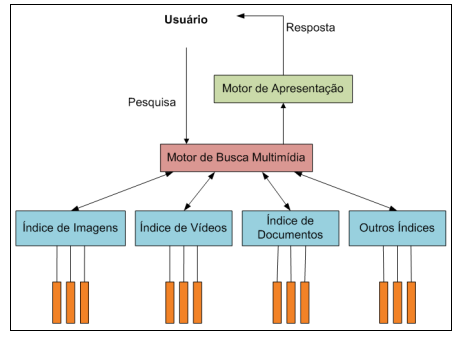
\includegraphics[width=0.6\textwidth]{Autonomia.png}
		\caption{Funcionamento do pincípio da autonomia .}
		\label{fig:exemplo1}
	\end{figure}
	
	\subsection{Princípio de Uniformidade}
	É usada uma única estrutura onde é indexado todos os tipos de mídia (imagem, vídeo, documento, auditivo, etc.). Essa abordagem demanda a análise do conteúdo de cada tipo de mídia para identificar características comuns entre os objetos, possibilitando a construção do índice. Sendo essa a forma mais simples de organização.
	
	\begin{figure}[ht]
		\centering
		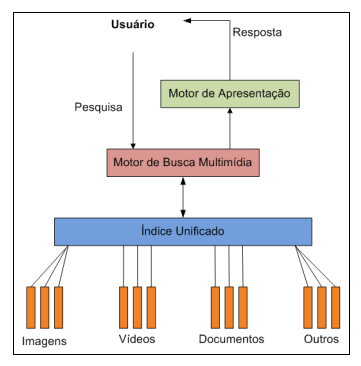
\includegraphics[width=0.6\textwidth]{Uniformidade.png}
		\caption{Funcionamento do pincípio da uniformidade.}
		\label{fig:exemplo2}
	\end{figure}
	
	\vspace{15em}
	
	\subsection{Princípio de Organização Híbrida}
	Uma terceira abordagem envolve a utilização do princípio híbrido. Segundo esse princípio, determinados tipos de mídia empregam índices individuais, ao passo que outros usam índices unificados. Dessa maneira, possuindo o melhor de cada arquitetura.
	
	\begin{figure}[ht]
		\centering
		\includegraphics[width=0.6\textwidth]{híbrido.png}
		\caption{Funcionamento do pincípio híbrido.}
		\label{fig3:exemplo3}
	\end{figure}
	
	%\vspace{10em}
	
	\section{Sistema de gerenciamento de banco de dados multimídia}
	
	O SGBD multimídia pode ser compreendido como o conjunto de processos empregados para definir, criar, armazenar, indexar, gerenciar e pesquisar em bancos de dados multimídia. Portanto, um   SGBDMM deve oferecer suporte para dados multimídia da mesma maneira que um SGBD tradicional suporta dados alfanuméricos simples.
	
	\subsection{Características de um SGBDMM}
	
	Um Sistema de Gerenciamento de Banco de Dados (SGBDMM) deve oferecer um ambiente diversificado e propício para a utilização e administração de bancos de dados multimídia, fornecendo suporte aos diferentes tipos de dados multimídia. As funções de um SGBDMM podem ser resumidas com base nas funções de um SGBD tradicional da seguinte maneira:
	
	\begin{itemize}
		
		\item \textbf{Integração de Dados}: Assegura que os elementos de dados armazenados não necessitem ser duplicados ao serem processados por diferentes programas.
		
		\item \textbf{Independência de Dados}: Permite a separação das funções que operam o SGBD e dos programas de aplicação. Ao garantir essa independência entre a lógica da aplicação e o armazenamento físico, são obtidos benefícios que possibilitam otimizar o armazenamento, a pesquisa e a recuperação dos dados, uma vez que o SGBD possui conhecimento sobre a estrutura e localização dos dados armazenados.
		
		\item  \textbf{Controle de Concorrência}: Em um  banco de dados multimídia assegura a consistência do banco. Essa garantia é alcançada por meio de regras que impõem ordem na execução de transações concorrentes. Como em um banco de dados multimídia as operações podem demorar muito, ele cria meios para facilitar esses processos. Como por exemplo ele pode dar o acesso apenas para a visualização e não para a alteração .
		
		\item \textbf{Persistência}: A persistência no contexto de objetos multimídia refere-se à capacidade desses objetos sobreviverem a transações e invocações realizadas por diferentes aplicações. Essa persistência é alcançada ao armazenar os arquivos multimídia em algum arquivo do sistema operacional. 
		
		
		\item \textbf {Controle de acesso}: Controla quem pode modificar o banco de dados.
		
		\item \textbf {Controle de integridade}: Garante a coerência dos dados armazenados em um banco de dados.
		
		\item \textbf{ Recuperação}: A garantia da recuperação no contexto de um banco de dados multimídia significa que falhas durante a execução de transações não devem afetar a durabilidade dos dados multimídia armazenados.
		
		\item \textbf {Processamento de pesquisa}: Assegurar que os mecanismos de pesquisa sejam adequados para dados multimídia é fundamental.No contexto multimídia, as operações de pesquisa e recuperação de dados tornam-se críticas e necessitam de eficiência e poder. Uma pesquisa típica pode abranger vários atributos, podendo ser baseada em palavras-chave ou orientada ao conteúdo, e frequentemente é interativa. A capacidade de realizar buscas eficazes e poderosas é crucial para explorar e acessar dados multimídia de maneira eficiente.
		
		\item \textbf{Controle de versão}: Organizar e gerenciar diversas versões dos objetos persistentes é crucial para atender às demandas de aplicativos que possam necessitar dessas diferentes versões.  A capacidade de manter e recuperar diferentes versões dos objetos contribui para a eficácia e flexibilidade do gerenciamento de dados multimídia.
		
	\end{itemize}
	
	\subsection{Requisitos para um SGBDMM}
	
	Como um sistema gerenciador de banco de dados multimídia pode ser muito heterogêneo, é essencial que o mesmo ofereça suporte a alguns requisitos básicos, tais como:
	
	\begin{itemize}
		
		\item \textbf {Métodos de indexação, pesquisa e organização dos dados
			multimídia}: Pois a pesquisa em banco de dados multimídia pode ser bastante trabalhosa, principalmente se for imagem ou vídeo onde o método de pesquisa utilizado for por conteúdo.
		
		\item \textbf { Sincronização e integração de diferentes tipos de dados multimídia}: A capacidade de lidar com solicitações assíncronas é uma característica crucial dos Sistemas de Gerenciamento de Bancos de Dados multimídia.
		
		\item \textbf{Linguagens formais de pesquisa em ambiente multimídia}: A linguagem empregada deve possuir a capacidade de expressar semântica complexa, bem como as relações temporais e espaciais associadas às informações multimídia compostas.
		
		\item \textbf {Estruturas eficientes de armazenamento de dados}: essas estruturas são necessárias para gerenciar dados multimídia.
		
		\item \textbf {Integração e suporte ao sistema operacional}: A arquitetura de um  SGBDMM e o sistema operacional precisam suportar o amplo conjunto de
		funcionalidades computacionais e a gerência dos dados.
		
		\item \textbf {Gerenciamento de bancos de dados multimídia distribuídos}: É essencial estabelecer coordenação e gerenciamento entre as localidades distribuídas para permitir o acesso transparente e rápido aos dados multimídia por diversos usuários.
		
		\item \textbf {Técnicas de modelagem formais para dados multimídia}: É a representação lógica e o relacionamento entre objetos multimídia, bem como as características que podem ser extraídas de cada objeto.
		
		\vspace{1em}
		
		Um modelo de dados multimídia deve capturar as seguintes informações \cite{debanco}:
		\vspace{1em}
		\item Detalhe da estrutura dos objetos multimídia;
		\item Operações pertinentes aos objetos multimídia;
		\item Propriedades dos objetos multimídia;
		\item Relacionamentos entre os objetos multimídia e os objetos do mundo real;
		\item Propriedades, relacionamentos e operações em objetos reais.
		
	\end{itemize}
	
	\section{Armazenamento de dados multimídia}
	\vspace{0.5 cm} \subsection{Referencias Externas}
	
	Nesse método de armazenamento, o banco de dados não tem controle direto sobre o objeto multimídia. O objeto é fisicamente armazenado fora do banco de dados, que mantém apenas uma referência ao local do objeto. Isso dificulta garantir consistência ou persistência dos dados, já que o banco de dados pode referenciar um objeto inexistente, ou o objeto pode não ter nenhum registro no banco de dados que o mencione.
	
	Porém, essa é a única forma de armazenamento que viabiliza acesso em tempo real ao objeto multimídia. Essa característica torna esse método adequado para aplicações que fornecem dados dos objetos conforme a necessidade do usuário, como aplicações de streaming que produzem objetos à medida que são lidos \cite{silva2006benchmark}.
	
	\subsection{Dados Multimídia Não Interpretados}
	
	Esse método de armazenamento utiliza campos do banco de dados para armazenar dados multimídia. No entanto, esses dados são tratados apenas como grandes sequências de bytes não interpretados, impossibilitando a extração direta das características semânticas dos objetos do campo \cite{silva2006benchmark}.
	
	Assim, o SGBD oferece apenas persistência, bufferização do acesso aos dados, suporte a multiusuário, recuperação e controle de autorização. Isso é diferente do armazenamento por referências externas, onde esses controles são viáveis. Sem mecanismos de abstração, desacoplar as aplicações multimídia da semântica dos dados não é possível. Assim, cada aplicação precisa implementar sua própria semântica (NUNES, p. 2).
	
	No contexto do armazenamento e recuperação de dados multimídia, é interessante observar que cada Sistema de Gerenciamento de Banco de Dados (SGBD) disponível no mercado tomou a iniciativa de desenvolver uma estrutura interna específica para lidar com esses tipos de dados. Essa abordagem personalizada reflete a diversidade de soluções e estratégias adotadas pelos diferentes SGBDs para otimizar o armazenamento e a recuperação eficientes de informações multimídia. Essas estruturas internas variam em termos de arquitetura e funcionalidades, refletindo a busca contínua por inovação e desempenho em um campo tão dinâmico como o gerenciamento de dados.
	
	\subsection{Funções Externas}
	
	Devido à limitação de recursos para manipular dados multimídia nos SGBDs, recorre-se a funções externas ao banco de dados. Essas funções externas são desenvolvidas ou empregadas para possibilitar extensões em linguagens de consulta e representação de objetos multimídia. Vale destacar que esse método de armazenamento também retém internamente o objeto multimídia \cite{silva2006benchmark}.
	
	\subsection{Orientação a Objetos}
	
	Nos sistemas orientados a objeto, é possível definir tipos de dados e referenciá-los na aplicação. Além disso, é viável construir hierarquias de tipos de dados, estabelecendo relacionamentos entre as classes correspondentes. Apesar dessas características, que tornam esse método de armazenamento uma das opções mais apropriadas, persistem desafios relacionados à gestão deficiente do acesso em tempo real \cite{silva2006benchmark}.
	
	\subsection{Comparativo Entre as Formas de Armazenamento}
	
	A Figura 4 apresenta uma comparação entre diversas formas de armazenamento de dados multimídia em um banco de dados, destacando as características distintas que cada uma possui.
	
	\begin{figure}[ht]
		\centering
		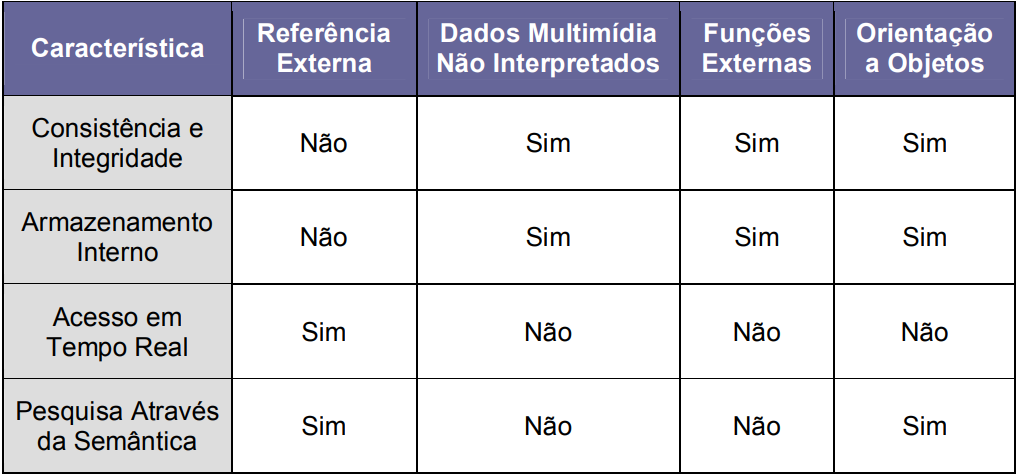
\includegraphics[width=0.7\linewidth]{image.jpg}
		\caption{Tabela de comparação}
		\label{fig:enter-label}
	\end{figure}
	
	\section{Aplicações de Banco de Dados Multimídia}
	
	As aplicações de bancos de dados multimídia podem variar amplamente em diferentes setores. Alguns exemplos dessas aplicações incluem:
	
	\begin{itemize}
		
		\item \textbf{Gestão de documentos e registros}: diversas indústrias e empresas mantêm registros detalhados, incluindo projetos de engenharia, dados de produção, registros médicos e documentos relacionados a prêmios de seguros;
		
		\item \textbf{Disseminação de conhecimento}: o uso de multimídia é uma maneira eficaz de disseminar conhecimento, promovendo o crescimento de recursos como livros, catálogos, manuais, enciclopédias eletrônicas e repositórios de informações;
		
		\item \textbf{Educação e treinamento}: o ensino de várias disciplinas para diferentes públicos, desde alunos do jardim-de-infância até treinamento de profissionais, pode ser projetado com recursos multimídia. A expectativa é de que bibliotecas digitais tenham uma influência significativa na forma como alunos, pesquisadores e outros usuários acessam extensos repositórios de materiais educacionais;
		
		\item \textbf{Marketing, propagandas, vendas no varejo, entretenimento e turismo}: informações multimídia são amplamente utilizadas nessas áreas, desde apresentações de vendas eficazes até experiências virtuais em cidades e galerias de arte. A indústria cinematográfica já demonstrou a eficácia dos efeitos especiais na criação de animações de animais, alienígenas e efeitos especiais artificialmente projetados. Além disso, a utilização de objetos armazenados pré-projetados em banco de dados multimídia ir á expandir a extensão dessas aplicações;
		
		\item \textbf{Controle e monitoramento em tempo real}: a apresentação multimídia de informações, em conjunto com tecnologias de banco de dados ativos, é eficiente para monitorar e controlar tarefas complexas, abrangendo operações de produção, usinas nucleares, unidades de terapia intensiva e sistemas de transporte.
		
	\end{itemize}
	
	\section{Conclusão}
	
	Em resumo, este trabalho oferece uma visão aprofundada dos desafios e potenciais dos bancos de dados multimídia. Ao abordar distinções entre dados convencionais e multimídia, princípios arquiteturais e estratégias de armazenamento, ele proporciona insights valiosos. A análise crítica das formas de armazenamento e requisitos de SGBDMM, juntamente com aplicações práticas, destaca a relevância e complexidade crescentes desses sistemas na era digital. Este trabalho serve como guia fundamental para compreender e explorar o papel dinâmico dos dados multimídia em diversos contextos.\vspace{1em}
	
	\bibliographystyle{sbc}
	\bibliography{sbc-template}
	
\end{document}